\chapter{Julia}

Julia es un lenguaje de programación gratis cuyo propósito general es ser tan rápido como C \val{Como pongo C? Así?}
pero manteniendo la facilidad de lenguaje de R o Python. Es una combinación de sintaxis simple con alto rendimiento computacional. Su slogan es "Julia se ve como Python, se siente como Lisp, corre como Fortran". [Hackers]. \val{Es un libro que todavia no está publicado, solo está en Gihub. Busco otro o como cito esto?}
Esta combinación de características hace que Julia sea un leguaje de programación que ha estado tomando mucha fuerza en la comunidad científica. Por lo tanto, en esta sección explicaré los básicos de Julia, desde su instalación hasta análisis de regresiones multivariadas. 

\section{Instalación}
Al momento de escritura de esta tesis la versión de Julia disponible es la v1.6.3 hasta el 23 de Septiembre del 2021. Para descargar Julia, hay que entrar al siguiente link: \url{https://julialang.org/downloads/}. 

\subsection{Windows}
\valinline{No se llama Ajustes, se llama Configuración}
Para esta versión de Julia, las opciones disponibles de descarga son un instalador de 64-bits o uno de 32-bits. Para saber el tipo de Sistema que tiene tu ordenador de Windows, debes seleccionar el botón de Start, después Ajustes > Sistema > Acerca de. En esta opción puedes ver el tipo de sistema que tiene tu computadora. Con esta información, eliges el instalador para tu computadora. Es importante seleccionar el "installer" y no el "portable". Una vez descargado, seleccionas el archivo .exe y sigues los pasos de instalación. 


\subsection{Mac}
\valinline{Qué tanto debo abarcar en Mac ya que yo tengo Windows?}
Para el sistema operativo de Mac, solo hay una versión disponible de descarga. Selecciona la opción de 64-bit. Una vez descargado, mueve el archivo de Julia al folder de \textquotedblleft Aplicaciones\textquotedblright. Para verificar que está bien descargado, haz click en el ícono de Julia y debe salir una terminal como la siguiente: \val{Puedo copiar una imagen que no sea mía, sino de una página web? referenciendola obvio}


\section{Atom}
Atom es un editor de texto de programación. Su meta es no comprometer hackabilidad y usabilidad \val{Suena horrible en español, en realidad es 'Our goal is a zero-compromise combination of hackability and usability'} \cite{ATOM}. Busca ser tán fácil para que cualquier persona, ya sea principiante o experto en la programación lo pueda utilizar. Por lo tanto, es una buena herramienta para escribir, editar y documentar el trabajo que uno hace en Julia. 

\subsection{Instalación en Windows} \val{Agrego la instalación en Mac?? No tengo Mac entonces todo sería de blogs}
Por supuesto, el primer paso es instalar el programa. Para hacerlo, hay que ir a la página \url{https://atom.io/} y hacer click en el botón de Download. \val{Otra vez palabra en inglés}

Una vez descargado el archivo ejecutable solo hay que darle click. Este proceso puede tardar un par de minutos. Sin embargo, una vez que termine el programa se ejecutará de manera automática. La pantalla se inicio se ve de la siguiente manera:

\begin{figure}[h]
\begin{center}
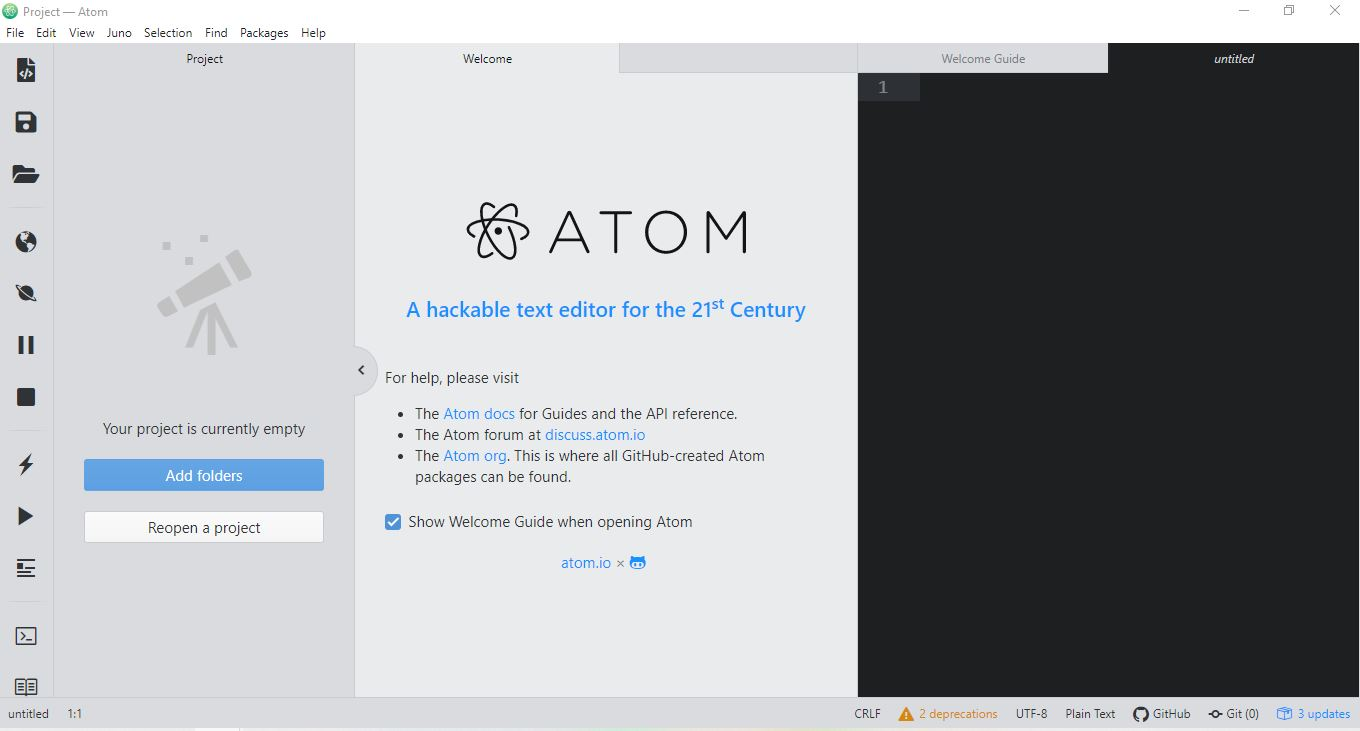
\includegraphics[scale=0.45]{Imagenes/atom_main_window.JPG}
 \caption{Ventana principal de Atom}
  \label{main_atom}
\end{center}
\end{figure}

El usuario puede modificar la pantalla de Atom con diferentes colores y temas siguiendo las instrucciones de la página \url{https://flight-manual.atom.io/getting-started/sections/atom-basics/}. Sin embargo, esa información no es relevante para esta tesis por lo que se va a omitir. 


\subsection{Conexión con Julia}
Ahora es momento de enlazar Julia con Atom. Para hacer esto, es necesario instalar el paquete Juno. 

\begin{enumerate}
    \item Abre Atom y selecciona File seguido de Settings. 
    \item En el panel izquierdo selecciona la opcion de Install y en el buscador de Install Packages escribe 'uber-juno'.
    \item Asegurate de que sea el paquete generado por JunoLab y haz click en el botón de Install. 
\end{enumerate}

Una vez instalado Juno, va a aparecer una opción llamada "Juno" en la parte superior de opciones entre "View" y "Selection". Para correr Julia dentro de Atom debes seleccionar Juno y después Open REPL. Aparecerá una nueva ventana en la parte inferior de la pantalla que te dirá que oprimas enter para iniciar una sesión de Julia. Después de hacerlo, Julia iniciará y podrás usarlo de manera normal. 
\\
Por otro lado, una ventaja de Atom es utilizarlo por su función principal: ser un editor de texto de programación. Es una forma fácil y rápida de crear código de Julia y el usuario puede decidir si correrlo dentro de Atom o directo en Julia. Para crear un nuevo archivo, hay que seleccionar la opción de File en la parte superior izquierda y después la opción de New File. Para que Atom reconozca ese archivo como texto del lenguaje Julia hay que guardarlo con el nombre deseado agregando '.jl' al final del nombre. 



\section{Símbolo del sistema}
Otra opción (y la favorita de la autora) es correr Julia desde el símbolo del sistema (también conocido como Command Prompt o cmd). \val{como digo palabras que estén en ingles? en italicas?} De ahora en adelante, se usarán por igual los términos símbolo del sistema y cmd.

\subsubsection{Agregar Julia a un PATH en Windows 10}

\valinline{Como referencio esta página? Es la oficial de Julia pero la estoy traduciendo y probando}

En ocasiones, después de haber instalado Julia podrías abrir el cmd de tu computadora, escribir 'julia' y aparecería una ventana como la siguiente: 

\begin{figure}[h]
\begin{center}
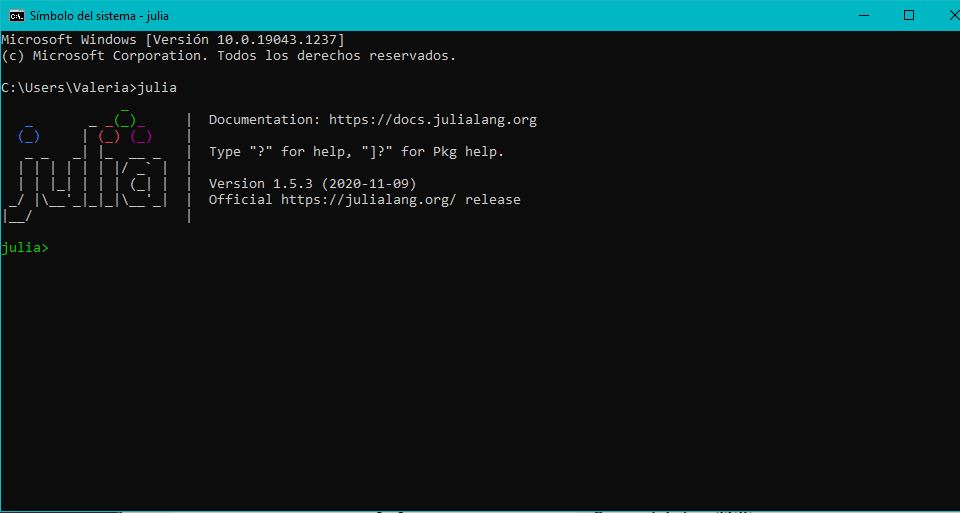
\includegraphics[scale=0.45]{Imagenes/julia_main_windows.JPG}
 \caption{Ventana principal de Julia}
  \label{main_Julia}
\end{center}
\end{figure}

En caso de que esto no ocurra, aparecerá un error en tu cmd que te dirá que no reconoce el comando 'julia' por lo que no lo puede ejecutar. En estos casos, los pasos a seguir son los siguientes:

\begin{enumerate}
    \item En el símbolo del sistema escribe 'rundll32 sysdm.cpl,EditEnvironmentVariables' y da click en el botón de Enter.
    \item Aparecerá una ventana nueva donde puedes editar las variables del usuario y las variables del sistema. En cualquiera de las dos opciones, selecciona la opción de 'Path' seguido de la opción 'Editar'. 
    \item En esta ventana nueva, selecciona la opción de 'Nuevo' y agrega el directorio de la instalación de Julia. En caso de no saberlo, escribe 'julia' en tu buscador de Windows y haz click en 'Abrir ubicación del archivo'. La dirección del programa debe ser algo similar a \path{C:\Users\Valeria\AppData\Local\Programs\Julia 1.5.3\bin}.
    \item Haz click en Aceptar, abre una nueva ventana de cmd y escribir julia debería funcionar. 
\end{enumerate}

Para más información sobre agregar un PATH en otras versiones de Windows, puedes consultar la siguiente página \url{https://julialang.org/downloads/platform/#windows}


\subsection{Threads}
Una de las razones por las que Julia es un lenguaje de programación muy rápido es que tiene la capacidad para multihilo (multithreading en inglés). Esto significa que puede correr diferentes tareas de manera simultánea en varios hilos. De la manera más simple: la meta de los autores de Julia fue hacer un lenguaje de programación con un rendimiento tan alto que pudiera hacer varias cosas a la vez. 
\\
Juno en Atom automáticamente pone la misma cantidad de hilos que la cantidad de núcleos de procesadores disponibles \cite{multithreading-julia}. Sin embargo, esto se puede modificar entrando a File > Settings > Packages. Después, buscar el paquete julia-client \val{otra palabra en ingles} y seleccionar los Settings del paquete. Finalmente, dentro del apartado de 'Julia Options' buscar 'Number of Threads' y poner el número deseado. 
\\
Por otro lado, si se está usando el símbolo de sistema el camino es diferente. Antes de ejecutar julia, es necesario modificar la cantidad de hilos que se van a utilizar. En Windows, \val{pongo Mac y Linux???} esto se hace escribiendo 'set JULIA\_ NUM\_ THREADS=4'. \val{Falta citar aquí el manual} En este ejemplo, se cambiaron los hilos a 4 pero se puede poner cualquier número.  \valinline{this is not necesarily true, cual es la cota superior????? FALTA BUSCAR} Después de hacer esta modificación, ahora sí ejecutamos julia. 
\\
Para observar que el cambio se ejecutó de manera correcta en cualquiera de las dos opciones basta con correr el comando 'Threads.nthreads()' y observar que la respuesta sea el número deseado. 


\section{Básicos de Julia}
Como ya se mencionó, Julia busca ser un lenguaje de programación sencillo e intuitivo. Por lo tanto, su sintáxis es bastante sencilla. La asignación de variables se hace con un signo de igualdad, $=$. El ejemplo más sencillo de esto sería $x = 2$ donde denotamos a x el valor de 2. 

\subsection{Operaciones básicas}
La siguiente tabla muestra la sintaxis usada para las operaciones básicas en Julia. 
\valinline{Dejo el screenshot referenciado o mejor hago una tabla yo solita y digo que toda la info la saque de la página oficial de julia?}

\begin{figure}[h]
\begin{center}
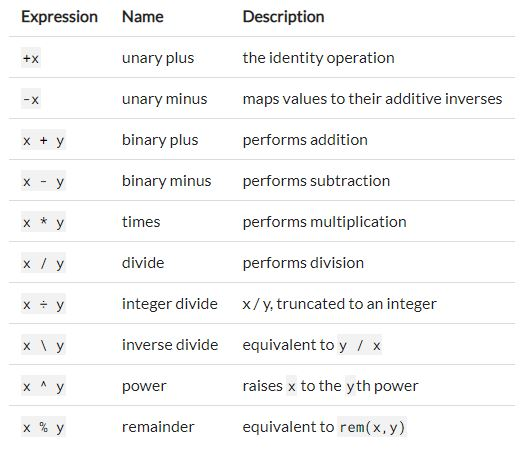
\includegraphics[scale=0.6]{Imagenes/operaciones_basicas_julia.JPG}
 \caption{Operaciones básicas en Julia. Fuente: \cite{Julia_manual}}
  \label{basic_operations_Julia}
\end{center}
\end{figure}

La siguiente tabla muestra los operadores booleanos en Julia. \val{Se ven horribles los \& \& pero no encuentro como arreglarlos}

\begin{center}
\begin{tabular}{ |c|c| } 
 \hline
 $!x$ & negación \\ 
 $x$ \& \& $y$ & operador de circuito corto $and$ \\ 
 $x \| y$ & operador de circuito corto $or$ \\ 
 \hline
\end{tabular}
\end{center}

\valinline{Además, como digo que esta tabla igual viene de \cite{Julia_manual} ?? }

\valinline{Me faltarían los vectorized 'dot' operations. Es que no sé que tanto profundizar aquí}

\valinline{Como no voy a estar manejando los imaginarios, no los pongo cierto?}

\subsection{Strings} \val{Debo de ponerlo todo en español I'm guessing. Tengo qe buscar un libro que me diga como se dice esto en español.}

Además de números, Julia puede asignar characteres a variables. Esto se hace utilizando las comillas dobles. Por ejemplo, 

\begin{figure}[h]
\begin{center}
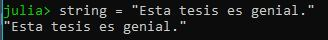
\includegraphics[scale=0.8]{Imagenes/ejemplo_string.JPG}
  \label{ejemplo_string_julia}
\end{center}
\end{figure}

Similar a otros lenguajes de programación, podemos accesar a caracteres específicos de un string utilizando corchetes cuadrados $[$ $]$ y a cadenas seguidas de caracteres usando $:$. Continuando con el ejemplo anterior, 
\begin{figure}[h]
\begin{center}
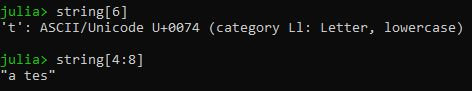
\includegraphics[scale=0.8]{Imagenes/ejemplo_string_partes.JPG}
  \label{ejemplo_string_julia_partes}
\end{center}
\end{figure}

Además, Julia también cuenta con la opción de concatenación de múltiples strings. Esto se hace utilizando un asterisco $*$ para separar cada uno de los strings. Por ejemplo,

\begin{figure}[h]
\begin{center}
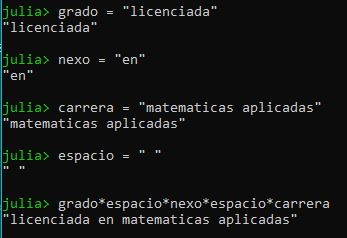
\includegraphics[scale=0.8]{Imagenes/ejemplo_concatenacion.JPG}
  \label{ejemplo_string_concatenacion}
\end{center}
\end{figure}

\subsection{Funciones}
En Julia, una función es un objeto que asigna una tupla de argumentos a un valor de retorno \cite{Julia_manual}. La sintáxis básica para definir funciones en Julia es:

\begin{figure}[h]
\begin{center}
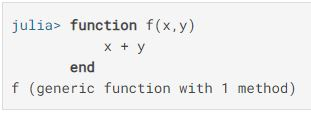
\includegraphics[scale=0.6]{Imagenes/sintaxis_funcion.JPG}
 \caption{Sintáxis básica de una función en Julia. Fuente: \cite{Julia_manual}}
  \label{functions_sintax_Julia}
\end{center}
\end{figure}

Además, puedes agregar la palabra $return$ para que la función regrese un valor. Por ejemplo, si quisieramos tener una función a la que les dos números y te regrese el número mayor, la sintaxis sería la siguiente:

\begin{figure}[h]
\begin{center}
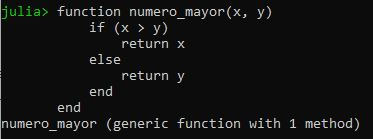
\includegraphics[scale=0.8]{Imagenes/ejemplo_return.JPG}
  \label{ejemplo_return}
\end{center}
\end{figure}

Para llamar a la función bastaría con escribir $numero_mayor(x, y)$ asignando o sustituyendo valores por $x$ y $y$. 

\subsection{Vectores y Matrices}

\begin{definition}
Un vector es un vector
\end{definition}

\subsection{DataFrames}

\subsection{Regresiones}
Pequeña intro a regresiones. Usar el paquete GLM que viene explicado en este link \url{https://juliastats.org/GLM.jl/stable/manual/}

\valinline{Que bases de datos voy a usar?}

\subsubsection{Regresión lineal simple}
Ver como salen los resultados aquí y si conviene o no graficar aquí o en R

\subsubsection{Histograma}

\subsubsection{Gráfica cuantil-cuantil}

\subsubsection{Análisis de residuales}

\subsubsection{Regresión lineal múltiple}

\subsubsection{Tabla de análisis de varianza}


\subsection{Paquete Distributions}
Para aprender como funcionan las distribuciones en Julia. El manual del paquete viene aquí \url{https://juliastats.org/Distributions.jl/v0.14/index.html}




